\documentclass[
  journal=largetwo,
  manuscript=original-article,
  year=2023-Submission,
  %volume=37,
]{cup-journal}

\usepackage{amsmath}
\usepackage[nopatch]{microtype}
\usepackage{lscape}
\newcommand{\blandscape}{\begin{landscape}}
\newcommand{\elandscape}{\end{landscape}}
\usepackage{longtable}
\usepackage{array}
\usepackage{wrapfig}
\usepackage{booktabs,
            makecell, multirow, tabularx}
\usepackage{colortbl}
\usepackage{pdflscape}
\usepackage{tabu}
\usepackage{threeparttable}
\usepackage{threeparttablex}
\usepackage[normalem]{ulem}
\usepackage{xcolor}
\usepackage{biblatex}
%\usepackage{natbib}

\title{Mapping psychological measures to adolescent AQoL-6D utility using data from young people attending primary mental health services}

\author{Matthew P Hamilton}
\affiliation{Orygen, Parkville, Australia}
\alsoaffiliation{School of Public Health and Preventive Medicine, Monash University, Clayton, Australia}

\author{Caroline X Gao}
\affiliation{Orygen, Parkville, Australia}
\alsoaffiliation{Centre for Youth Mental Health; University of Melbourne, Parkville, Australia}
\alsoaffiliation{School of Public Health and Preventive Medicine, Monash University, Clayton, Australia}
\email[Caroline X Gao]{caroline.gao@orygen.org.au}

\author{Kate M Filia}
\affiliation{Orygen, Parkville, Australia}
\alsoaffiliation{Centre for Youth Mental Health; University of Melbourne, Parkville, Australia}

\author{Jana M Menssink}
\affiliation{Orygen, Parkville, Australia}
\alsoaffiliation{Centre for Youth Mental Health; University of Melbourne, Parkville, Australia}

\author{Sonia Sharmin}
\affiliation{Orygen, Parkville, Australia}
\alsoaffiliation{Centre for Youth Mental Health; University of Melbourne, Parkville, Australia}

\author{Sonia Sharmin}
\affiliation{Orygen, Parkville, Australia}
\alsoaffiliation{Centre for Youth Mental Health; University of Melbourne, Parkville, Australia}

\author{Nic Telford}
\affiliation{headspace National Youth Mental Health Foundation, Melbourne, Australia}

\author{Helen Herrman}
\affiliation{Orygen, Parkville, Australia}
\alsoaffiliation{Centre for Youth Mental Health; University of Melbourne, Parkville, Australia}

\author{Ian B Hickie}
\affiliation{Brain and Mind Centre, Youth Mental Health \& Technology, Faculty of Medicine \& Health, The University of Sydney, Australia}

\author{Cathrine  Mihalopoulos}
\affiliation{School of Public Health and Preventive Medicine, Monash University, Clayton, Australiae}

\author{Debra J Rickwood}
\affiliation{Faculty of Health, University of Canberra, Australia}
\alsoaffiliation{headspace National Youth Mental Health Foundation, Melbourne, Australia}

\author{Patrick D McGorry}
\affiliation{Orygen, Parkville, Australia}
\alsoaffiliation{Centre for Youth Mental Health; University of Melbourne, Parkville, Australia}

\author{Sue M Cotton}
\affiliation{Orygen, Parkville, Australia}
\alsoaffiliation{Centre for Youth Mental Health; University of Melbourne, Parkville, Australia}

\addbibresource{RefCopy.bib}

\keywords{anxiety, AQoL, depression, psychological distress, QALYs, utility mapping} %% First letter not capped

\begin{document}

\begin{abstract}
\textit{Background: } Quality Adjusted Life Years (QALYs) are often used in economic evaluations, yet utility weights for deriving them are rarely directly measured in mental health services.
\textit{Objectives: } We aimed to identify the best mapping models and predictors for adolescent Assessment of Quality of Life - Six Dimensions (AQOL-6D) utility and assess the ability of mapping models to predict longitudinal change.
\textit{Methods: } We recruited 1107 young people attending Australian primary mental health services, collecting data at two time points, three months apart. Five linear and three generalised linear models were explored to identify the best mapping model. Ten-fold cross-validation using R\(^2\), root mean square error (RMSE) and mean absolute error (MAE) were used to compare models and assess predictive ability of six candidate measures of psychological distress, depression and anxiety. Linear / generalised linear mixed effect models were used to construct longitudinal predictive models for AQoL-6D change.
\textit{Results: } A depression measure (Patient Health Questionnaire-9) was the strongest independent predictor of health utility. Linear regression models with complementary log-log transformation of utility score were the best performing models. Between-person associations were slightly larger than within-person associations for most of the predictors.
\textit{Conclusions: } Adolescent AQoL-6D utility can be derived from a range of psychological distress, depression and anxiety measures. Mapping models estimated from cross-sectional data can approximate longitudinal change but may slightly bias health utility predictions.
\textit{Data: } Replication code, detailed results and guidance on how to apply the models produced by this study are available in the online repository: \url{https://doi.org/10.7910/DVN/DKDIB0}.
\end{abstract}

\section{Introduction}

Quality adjusted life years (QALYs) are generic indices of outcome that inform public health policy in many countries \autocite{RN3417}. One of the main uses of QALYs is as the measure of benefit in Cost-Utility Analyses (CUAs). Compared to economic evaluations that use other outcome measures, CUAs facilitate comparisons of the value for money claims of interventions for different health conditions. CUAs have this advantage because QALYs can measure outcomes in populations from diverse illness groups and are associated with well understood policymaker willingness to pay thresholds.

The ``quality'' in QALYs is measured via the use of multi-attribute utility instruments (MAUIs), where domains of quality of life measured by a questionnaire are weighted using people's preferences \autocite{RN3418}. This approach produces a single health utility value for each individual for each measured health state, anchored on a scale where 0 represents a state equivalent to death and 1 represents perfect health. Health utilities can be converted to QALYs by weighting the duration (the ``years'' part of QALYs) each individual spends in each health state.

MAUIs are regularly used in research studies such as clinical trials and epidemiological surveys, but rarely feature in routine data collection by mental health services. In the absence of direct measurement, mapping analysis has been developed to predict health utility from standard health status measurements \autocite{RN7,Wailoo2017}. MAUIs such as the Assessment of Quality of Life -- 8 dimensions (AQoL-8D \autocite{Richardson2014}) have been shown to be sensitive to psychological distress and depression measures \autocite{RN6} and can be mapped to \autocite{RN4} using measures of psychological distress (measured using Kessler Psychological Distress Scale -- 10 items, K10 \autocite{RN16}) and depression and anxiety symptoms (measured using Depression, Anxiety, and Stress Scale -- 21 items, DASS-21 \autocite{henry_2005}). However, it is unclear which mental health measures are the most predictive of health utility and existing algorithms developed for adult \autocite{RN4} or child \autocite{pmid23943259} general populations are of questionable appropriateness for predicting health utility in clinical youth mental health samples.

Currently available mapping algorithms are largely derived from cross-sectional data and assume that the associations between psychological measurements and health utility are time-invariant. Therefore, the between-person association (variations in mental health symptoms associated with variations in health utility observed cross-sectionally in a population) can be applied to estimate the within-person association (changes in mental health symptoms associated with changes in health utility over time). However, this time invariant assumption may not be true (for example, health utility measures may be less sensitive to change compared with measures of mental health symptoms).

To facilitate cost-utility analyses of primary youth mental health services, we aimed to use data from a sample of help-seeking young people to: (i) identify the best mapping regression models to predict adolescent weighted AQoL-6D utility from six candidate measures of psychological distress, depression and anxiety; and (ii) assess ability of the mapping algorithms to predict longitudinal (three-month) change.

\section{Methods}

\subsection{Ethics approval}

The study was approved by the University of Melbourne's Human Research Ethics Committee and the local Human Ethics and Advisory Group (1645367.1)

\subsection{Sample and setting}

This study forms part of a youth outcomes measurement research program, and the study sample has previously been described \autocite{Filia_2021}. Briefly, young people aged 12 to 25 years who presented for a first appointment for mental health or substance use related issues were recruited from three metropolitan and two regional Australian youth-focused primary mental health clinics (headspace centres) between September 2016 to April 2018. Sample characteristics are similar to previous descriptions of headspace clients, with slight differences in age (less aged 12-14, more aged 18-20), cultural background (more Culturally and Linguistically Diverse and less Aboriginal and Torres Strait Islander young people), sexuality (fewer heterosexual clients) and housing (more in unstable accommodation) \autocite{Filia_2021}.

\subsection{Measures}

We collected data on health utility, six candidate predictors of health utility including psychological distress, depression and anxiety measures as well as demographic, clinical and functional population information.

\subsubsection{Health utility}

We assessed health utility using the adolescent version of the Assessment of Quality of Life -- Six Dimension scale (AQoL-6D; \autocite{RN10}) MAUI. It was selected due to its validity for use in adolescents, the relevance of its domains for a clinical mental health sample \autocite{RN6} and its acceptable participant time-burden. The AQoL-6D instrument contains 20 items across the six dimensions of independent living, social and family relationship, mental health, coping, pain and sense. Health utility scores were calculated using a published algorithm (available at \url{https://www.aqol.com.au/index.php/aqolinstruments?id=92}), using Australian population preference weights. The distribution of AQoL-6D instrument item specific scores within our sample has been described in a previous study \autocite{cotton_hamilton_filia_2022}.

\subsubsection{Candidate predictors}

Data from six measures of psychological distress (one measure), depression (two measures) and anxiety (three measures) symptoms were used as candidate predictors to construct mapping models. These measures are widely used in clinical mental health services or clinically relevant to the profiles of young people seeking mental health care.

The Kessler Psychological Distress Scale (K6; \autocite{RN16}) was used to measure psychological distress over the last 30 days. It includes six items (nervousness, hopelessness, restlessness, sadness, effort, and worthlessness) of the 10 item version of this measure, K10. Individual items use a five-point frequency scale that spans from 0 (``none of the time'') to 4 (``all of the time'').

The Patient Health Questionnaire-9 (PHQ-9; \autocite{RN11}) and Behavioural Activation for Depression Scale (BADS; \autocite{RN12}) were used to measure degree of depressive symptomatology. PHQ-9 includes nine questions measuring the frequency of depressive thoughts (including self-harm/suicidal thoughts) as well as associated somatic symptoms (e.g., sleep disturbance, fatigue, anhedonia, appetite, psychomotor changes) in the past two weeks. PHQ-9 uses a four-point frequency scale ranging from 0 (``Not at all'') to 3 (``Nearly every day''). For the PHQ-9 a total score is derived (0-27) with higher scores depicting greater symptom severity. BADS measures a range of behaviours (activation, avoidance/rumination, work/school impairment as well as social impairment) reflecting severity of depression. BADS includes 25 questions on behaviours over the past week, scored on a seven-point scale ranging from 0 (``Not at all'') to 6 (``Completely''). A total score is derived for the BADS (0-150) as well as subscale scores, with higher scores indicating greater activation.

The Generalised Anxiety Disorder Scale (GAD-7; \autocite{RN13}), Screen for Child Anxiety Related Disorders (SCARED; \autocite{RN14}) and Overall Anxiety Severity and Impairment Scale (OASIS; \autocite{RN15}) were used to measure anxiety symptoms. GAD-7 measures symptoms such as nervousness, worrying and restlessness, over the past two weeks using seven questions, with a four-point frequency scale ranging from 0 (``Not at all'') to 3 (Nearly every day''). A total score is calculated with scores ranging from 0 to 21 and higher scores indicating more severe symptomatology. SCARED is an anxiety screening tool designed for children and adolescents which can be mapped directly on specific Diagnostic and Statistical Manual of Mental Disorders (DSM-IV-TR) anxiety disorders including generalised anxiety disorder, panic disorder, separation anxiety disorder and social phobia. It includes 41 questions on a three-point scale of 0 (``Not true or hardly ever true''), 1 (``Somewhat True or Sometimes True'') and 2 (``Very true or often true'') to measure symptoms over the last three months. A total score is derived with scores ranging from 0-82, with higher scores indicative of the presence of an anxiety disorder. The OASIS was developed as a brief questionnaire to measure severity of anxiety and impairment in clinical populations. The OASIS includes five questions about frequency and intensity of anxiety as well as related impairments such as avoidance, restricted activities and problems with social functioning over the past week. Total scores range from 0-20 with higher scores depicting more severe symptomatology.

\subsubsection{Population characteristics}

We collected self-reported demographic measures (age, gender, sex at birth, education and employment status, languages spoken at home and country of birth). We also collected clinician or research interviewer assessed measures of mental health including primary diagnosis, clinical stage \autocite{McGorry_2006} and functioning (measured by the Social and Occupational Functioning Assessment Scale (SOFAS) \autocite{Goldman_1992}).

\subsection{Procedures}

Eligible participants were recruited by trained research assistants and responded to the questionnaire via a tablet device. Participants' clinical characteristics were obtained from clinical records and research interview. At three-months post-baseline, participants were contacted in person or by telephone, to complete a follow-up assessment.

\subsection{Statistical analysis}

We undertook a three-step process to: i) gain insight into our dataset and measures; ii) specify models and assess model performance using cross-sectional data; and iii) specify longitudinal models and assess whether modelling assumptions were met.

\subsubsection{Pre-modelling steps}

Basic descriptive statistics characterised the cohort in terms of baseline demographics and clinical variables. Pearson's Product Moment Correlations (\emph{r}) were used to determine the relationships between candidate predictors and AQoL-6D utility score.

\subsubsection{Cross-sectional model specification and assessment}

Good practice guidance on mapping studies \autocite{Wailoo2017} does not advocate specific model types as the appropriate choice will vary depending on factors that include the health utility measure being mapped to, the applicable health condition and target population, the clinical variables used as predictors and the intended use of the mapping algorithm. Compared to the EQ-5D utility measures most commonly used in the mapping literature \autocite{Mukuria2019}, AQOL-6D has better dimensional overlap with mental health measures \autocite{RN6} and is derived from a greater number of questionnaire items (which can generate more continuous utility score distributions). The types of models we explored reflected these considerations.

We used a cross-section of our dataset (baseline measures only) to explore appropriate type(s) of models to use, compare the relative predictive performance of candidate predictors, and identify other potential risk factors associated with quality of life independent of mental health measures.

As AQoL-6D utility score is normally left skewed and constrained between 0 and 1, ordinary least squares (OLS) models with different types of outcome transformations (such as log and logit) have been previously used in mapping \autocite{RN7}. Similarly, generalised linear models (GLMs) address this issue via modelling the distribution of the outcome variable and applying a link function between the outcome and linear combination of predictors \autocite{Dobson_2018}. Beta regressions, which can be considered a special form of GLMs, are another popular strategy for modelling health utility \autocite{Hunger2011}.

We chose to explore OLS, GLM and beta models with commonly adopted transformation algorithms. The models we selected for comparison were OLS regression with log, logit, log-log (\(f(y) = -log(-log(y))\)) and clog-log (\(f(y) = log(-log(1-y))\)) transformation; GLM using Gaussian distribution with log link; and beta regression with logit and clog-log link. For each candidate model type, we evaluated the modelling performance and predictive ability of a univariate model using the candidate predictor with the highest Pearson correlation coefficient with utility scores. Ten-fold cross-validation was used to compare model fitting using training datasets and predictive ability using testing datasets using three indicators including R\^{}2, root mean square error (RMSE) and mean absolute error (MAE) \autocite{RN20,RN19}. After identifying the best performing model type, we used 10-fold cross-validation to compare predictive ability of six mental health measures in predicting AQol-6D (one model for each candidate predictor).

To evaluate whether candidate predictors could independently predict utility scores, we added a range of independent variables to each of the six models that included participants' age, sex at birth, clinical stage, cultural and linguistic diversity, education and employment status, primary diagnosis, region of residence (whether metropolitan - based on location of attending service) and sexual orientation. Functioning (as measured by SOFAS) was also included in each model to evaluate whether it can jointly predict utility with clinical symptom measurements.

\subsubsection{Longitudinal modelling and assumption testing}

After identifying the best mapping regression model(s) for predicting between person change, we established longitudinal models to predict within person change. This was achieved using generalised linear mixed- effect models (GLMM) including both the baseline and follow-up data. All records with complete baseline data (with or without follow-up data) were included.

Bayesian linear mixed models were used to avoid common convergence problems in frequentist tools \autocite{bolker2009generalized}. Linear mixed effect model (LMM) can be fitted in the same framework with Gaussian distribution and identify link function. Clustering at individual level is controlled via including random intercepts. Model fitting was evaluated using Bayesian R\textsuperscript{2} \autocite{RN21}.

We compared the model coefficients for each predictor's score at baseline and score change from baseline to assess the potential bias of estimating score changes within individuals using score difference between individuals.

\subsection{Replicability}

We undertook all our analyses using \textbf{\emph{R}} 4.0.5 \autocite{RCitation}, using a wide range of packages (see Online Supplement, A.5). To aid study replication and appropriate out of sample use of our mapping models, we developed R packages, programs and reporting templates, which we disseminated along with data and documentation in online repositories (see Data Availability Statement).

\section{Results}

\subsection{Cohort characteristics}

Participants characteristics are summarised in Table \ref{tab:participantstb}. This study included 1068 (out of the 1073) participants with complete AQoL-6D data at baseline. This cohort predominantly comprised individuals with anxiety/depression (76.650\%) at early (prior to first episode of a serious mental disorder) clinical stages (91.707\%). Participant ages ranged between 12-25 with a mean age of 18.129 (SD = 3.263).

There were 643 participants (60.205\%) who completed AQoL-6D questions at the follow-up survey.

\subsection{AQoL-6D and candidate predictors}

Distributions of AQoL-6D total utility score and sub-domain scores are displayed in Figure \ref{fig:fig1}. The mean utility score at baseline is 0.589 (SD = 0.235) and is 0.678 (SD = 0.238) at follow-up. Distributions of candidate predictors, K6, BADS, PHQ-9, GAD-7, OASIS and SCARED, are summarised in Table \ref{tab:predrscors}. PHQ-9 was found to have the highest correlation with utility score both at baseline and follow-up followed by OASIS and BADS; baseline and follow-up SCARED was found to have the lowest correlation coefficients with utility score, although all correlation coefficients can be characterised as strong.

\subsection{Cross-sectional models}

The 10-fold cross-validated model fitting indices from mapping models using PHQ-9 are reported in Online Supplement Table A.1. There were convergence issues with beta regression models and, as they do not show major advantages in predictive performance, these models were not considered further.

Model diagnoses (such as heteroscedasticity, residual normality) suggested better model fit of the clog-log transformed OLS model, as the distribution of clog-log transformed utility are closest to normal distribution among all transformation methods. Another benefit of the clog-log transformed model is that the predicted utility score will be constrained with an upper bound of 1, thus preventing out of range prediction. Therefore, OLS with clog-log transformation was chosen as the best model for further evaluation. The GLM with Gaussian distribution and log link is commonly used in mapping studies \autocite{Mukuria2019}, so was included to provide comparisons with other published work.

PHQ9 had the highest predictive ability followed by OASIS, BADS, GAD7 and K6 (Online Supplement Table A.2 ). SCARED had the least predictive capability. The confounding effect of other participant characteristics were also evaluated, with SOFAS found to independently predict utility scores in models for all six candidate predictors (\emph{p\textless0.005}). Sex at birth was found to be a confounder for the K6 model (\emph{p\textless0.01}). A few other confounders, including primary diagnosis, clinical staging and age were identified as weakly associated with utility in mapping models using anxiety and depression measurements other than PHQ-9. Many of these factors are unlikely to change over three months, so were not evaluated in the mixed effect models.

\subsection{Longitudinal models}

Regression coefficients of the baseline score and score changes (from baseline to follow-up) estimated in individual GLMM and LMM models are summarised in Table \ref{tab:cfscl}. In GLMM and LMM models, the prediction models using OASIS and PHQ-9 respectively had the highest R\textsuperscript{2} (0.681 and 0.762). R\textsuperscript{2} was between 0.581 and 0.681 for all GLMMs and between 0.712 and 0.762 for all LMMs.. Variance of the random intercept was comparable with the residual variance.

Distribution of observed and predicted utility scores and their association from GLMM (Gaussian distribution with log link) and LMM (c-loglog transformed) using PHQ-9 are plotted in Figure \ref{fig:fig2}. Compared with GLMM, the predicted utility scores from LMM converge better to the observed distribution and provide better estimations at the tail of the distribution. When the observed utility scores were low, the predicted utility were too high in the GLMM model, see Figure 2 (B). The observed and predicted distributions of utility scores for other anxiety and depression measurements were similar for LMM. However, GLM had low coverage in utility scores below 0.3 and also made predictions out of range (over 1).

Model coefficients of score change from baseline were generally estimated to be lower compared with coefficients of baseline score (except for SCARED). The mean (across GLMM and LMM models) ratio of the two coefficients (\({\beta}_{change}/{\beta}_{baseline}\)) is 0.823 for K6, between 0.802 and 0.850 for depression measurements and between 0.900 and 1.086 for anxiety measurements.

\section{Discussion}

Although there is encouraging evidence about the quality, effectiveness and cost-effectiveness of youth mental health service innovations worldwide \autocite{RN1027,RN1033}, the public health and economic returns from systemic reforms to support better mental health in young people needs to be better understood \autocite{RN1043}. Our study contributes to this goal by developing tools that can facilitate derivation of QALYs from measures commonly collected in youth mental health services.

Our study is the first to evaluate longitudinal mapping ability between a wide range of affective symptom measurements and health utility in a cohort of help seeking young people. We were able to independently predict adolescent AQoL-6D from each of the six candidate measures we assessed, with PHQ-9 having the best predictive performance. Predictive performance was improved when adding a measure of functioning (SOFAS) as an additional predictor or confound to each model; SOFAS also performed well as an independent predictor. As many youth mental health services routinely collect data on at least one of the predictors included in our models, these mapping models may have widespread applicability.

Study results may be useful for helping service system planners to prioritise the measures to include in routine data collection. Although direct measurement of health utility with measures such as the ReQoL \autocite{KEETHARUTH2021281} may be feasible in some mental health services, relying on clinical measures that can also map to health utility may be an attractive alternative.

A key feature of QALYs is their longitudinal dimension - health utilities are weighted and aggregated based on the time spent in varying health states. Our results suggest that cross-sectional variations in psychological distress, depression and anxiety measurements can be used to approximate the longitudinal change in health utility in this cohort. However, for psychological distress and depression measures at least, mapping algorithms developed from cross-sectional data may slightly over-estimate these changes, introducing bias into QALY predictions (overestimating QALYs for populations whose health utility improves over time, underestimating QALYs for those with deteriorating mental health).

Key strengths of our study include the novelty of our clinical youth mental health study sample, the use of clinically relevant and frequently collected outcome measures as predictors, the appropriateness and range of statistical methods deployed, the comparison of within-person and between-person differences in health utility weight predictions and highly replicable, publicly disseminated study algorithms. We acknowledge limitations that our data pertained to a single country, and we explored only one MAUI-derived utility weight. However, using utility weight input data derived from the same country as that to which an analysis pertains may be relatively unimportant \autocite{homecountryhypo}, particularly when the MAUI is well suited to the relevant health condition (as is the case with AQoL and mental health \autocite{RN6}). We did not examine some potential predictors that may be more common in some mental health services (for example we explored K6, as opposed to the expanded, and commonly used measure, the K10). We also did not develop age-group specific models which would be a potentially useful extension of this work.

\section{Conclusions}

We have found that it is possible to predict both within-person and between-person differences in adolescent AQOL-6D utility weights from measures routinely collected in youth mental health services. Mapping algorithms developed from cross-sectional data can approximate longitudinal changes in health utility, but may slightly over-estimate these changes. The mapping algorithms we have developed can enable greater use of CUAs in economic evaluations using youth mental health data collections.

\paragraph{Funding Statement}

The study was funded by the National Health and Medical Research Council (NHMRC, APP1076940), Orygen and headspace.

\paragraph{Competing Interests}

None declared.

\paragraph{Data Availability Statement}

Utility mapping models, instructions on how to apply them and study replication code are distributed as part of the study data repository (\url{https://doi.org/10.7910/DVN/DKDIB0}). R packages are available for replicating and transferring study methods (\url{https://ready4-dev.github.io/TTU/}) and applying the mapping models to out of sample data (\url{https://ready4-dev.github.io/youthu/)}.

\printendnotes

\printbibliography

\clearpage

\appendix

\begin{table*}

\caption{\label{tab:participantstb}Participant characteristics}
\centering
\begin{tabular}[t]{>{\raggedright\arraybackslash}p{14em}l>{\raggedright\arraybackslash}p{6em}>{\raggedright\arraybackslash}p{6em}>{\raggedright\arraybackslash}p{6em}>{\raggedright\arraybackslash}p{6em}}
\toprule
\multicolumn{1}{c}{ } & \multicolumn{1}{c}{ } & \multicolumn{2}{c}{Baseline} & \multicolumn{2}{c}{Follow-Up} \\
\cmidrule(l{3pt}r{3pt}){3-4} \cmidrule(l{3pt}r{3pt}){5-6}
 &  & (N = & 1068) & (N = & 643)\\
\midrule
 & Mean (SD) & 18.129 & (3.263) & 18.191 & (3.249)\\
\cmidrule{2-6}
 & Median (Q1\, Q3) & 18.000 & (16.000\, 20.000) & 18.000 & (16.000\, 21.000)\\
\cmidrule{2-6}
 & Min - Max & 12.000 & 25.000 & 12.000 & 25.000\\
\cmidrule{2-6}
\multirow{-4}{14em}{\raggedright\arraybackslash \textbf{Age}} & Missing & 0.000 &  & 0.000 & \\
\cmidrule{1-6}
 & Female & 653.000 & (62.131\%) & 398.000 & (63.175\%)\\
\cmidrule{2-6}
 & Male & 359.000 & (34.158\%) & 207.000 & (32.857\%)\\
\cmidrule{2-6}
 & Other & 39.000 & (3.711\%) & 25.000 & (3.968\%)\\
\cmidrule{2-6}
\multirow{-4}{14em}{\raggedright\arraybackslash \textbf{Gender}} & Missing & 17.000 &  & 13.000 & \\
\cmidrule{1-6}
 & Not in relationship & 695.000 & (66.699\%) & 426.000 & (68.269\%)\\
\cmidrule{2-6}
 & In relationship & 347.000 & (33.301\%) & 198.000 & (31.731\%)\\
\cmidrule{2-6}
\multirow{-3}{14em}{\raggedright\arraybackslash \textbf{Relationship status}} & Missing & 26.000 &  & 19.000 & \\
\cmidrule{1-6}
 & Heterosexual & 738.000 & (71.860\%) & 431.000 & (69.516\%)\\
\cmidrule{2-6}
 & Other & 289.000 & (28.140\%) & 189.000 & (30.484\%)\\
\cmidrule{2-6}
\multirow{-3}{14em}{\raggedright\arraybackslash \textbf{Sexual orientation}} & Missing & 41.000 &  & 23.000 & \\
\cmidrule{1-6}
 & Metro & 671.000 & (62.828\%) & 382.000 & (59.409\%)\\
\cmidrule{2-6}
 & Regional & 397.000 & (37.172\%) & 261.000 & (40.591\%)\\
\cmidrule{2-6}
\multirow{-3}{14em}{\raggedright\arraybackslash \textbf{Region of residence}} & Missing & 0.000 &  & 0.000 & \\
\cmidrule{1-6}
 & Studying only & 405.000 & (39.093\%) & 247.000 & (39.711\%)\\
\cmidrule{2-6}
 & Working only & 167.000 & (16.120\%) & 91.000 & (14.630\%)\\
\cmidrule{2-6}
 & Studying and working & 305.000 & (29.440\%) & 193.000 & (31.029\%)\\
\cmidrule{2-6}
 & Not studying or working & 159.000 & (15.347\%) & 91.000 & (14.630\%)\\
\cmidrule{2-6}
\multirow{-5}{14em}{\raggedright\arraybackslash \textbf{Education and employment status}} & Missing & 32.000 &  & 21.000 & \\
\cmidrule{1-6}
 & Depression & 182.000 & (17.931\%) & 108.000 & (17.308\%)\\
\cmidrule{2-6}
 & Anxiety & 264.000 & (26.010\%) & 181.000 & (29.006\%)\\
\cmidrule{2-6}
 & Depression and Anxiety & 332.000 & (32.709\%) & 188.000 & (30.128\%)\\
\cmidrule{2-6}
 & Other & 237.000 & (23.350\%) & 147.000 & (23.558\%)\\
\cmidrule{2-6}
\multirow{-5}{14em}{\raggedright\arraybackslash \textbf{Primary diagnosis}} & Missing & 53.000 &  & 19.000 & \\
\cmidrule{1-6}
 & 0-1a & 625.000 & (60.270\%) & 456.000 & (72.038\%)\\
\cmidrule{2-6}
 & 1b & 326.000 & (31.437\%) & 131.000 & (20.695\%)\\
\cmidrule{2-6}
 & 2-4 & 86.000 & (8.293\%) & 46.000 & (7.267\%)\\
\cmidrule{2-6}
\multirow{-4}{14em}{\raggedright\arraybackslash \textbf{Clinical stage}} & Missing & 31.000 &  & 10.000 & \\
\cmidrule{1-6}
 & Mean (SD) & 65.182 & (9.479) & 69.901 & (10.082)\\
\cmidrule{2-6}
 & Median (Q1\, Q3) & 65.000 & (60.000\, 72.000) & 70.000 & (64.000\, 78.000)\\
\cmidrule{2-6}
 & Min - Max & 29.000 & 90.000 & 20.000 & 91.000\\
\cmidrule{2-6}
\multirow{-4}{14em}{\raggedright\arraybackslash \textbf{Social and Occupational Functioning Assessment Scale}} & Missing & 30.000 &  & 7.000 & \\
\bottomrule
\end{tabular}
\end{table*}

\begin{table*}

\caption{\label{tab:predrscors}Candidate predictors distribution parameters and correlations with AQoL-6D utility}
\centering
\begin{tabular}[t]{>{\raggedright\arraybackslash}p{14em}l>{\raggedright\arraybackslash}p{3em}>{\raggedright\arraybackslash}p{3em}>{\raggedright\arraybackslash}p{3em}>{\raggedright\arraybackslash}p{3em}l}
\toprule
\multicolumn{1}{c}{ } & \multicolumn{1}{c}{ } & \multicolumn{2}{c}{Baseline} & \multicolumn{2}{c}{Follow-Up} & \multicolumn{1}{c}{ } \\
\cmidrule(l{3pt}r{3pt}){3-4} \cmidrule(l{3pt}r{3pt}){5-6}
 &  & (N = & 1068) & (N = & 643) & \textit{p}\\
\midrule
 & Mean (SD) & 78.158 & (24.823) & 89.360 & (24.435) & 0.000\\
\cmidrule{2-7}
 & Missing & 10.000 &  & 2.000 &  & 0.000\\
\cmidrule{2-7}
\multirow{-3}{14em}{\raggedright\arraybackslash \textbf{Behavioural Activation for Depression Scale (0-150)}} & Correlation with AQOL-6D & 0.665 &  & 0.659 &  & 0.000, 0.000\\
\cmidrule{1-7}
 & Mean (SD) & 10.382 & (5.658) & 7.945 & (5.460) & 0.000\\
\cmidrule{2-7}
 & Missing & 6.000 &  & 2.000 &  & 0.000\\
\cmidrule{2-7}
\multirow{-3}{14em}{\raggedright\arraybackslash \textbf{Generalised Anxiety Disorder Scale (0-21)}} & Correlation with AQOL-6D & -0.653 &  & -0.685 &  & 0.000, 0.000\\
\cmidrule{1-7}
 & Mean (SD) & 12.156 & (5.765) & 9.811 & (5.873) & 0.000\\
\cmidrule{2-7}
 & Missing & 4.000 &  & 2.000 &  & 0.000\\
\cmidrule{2-7}
\multirow{-3}{14em}{\raggedright\arraybackslash \textbf{Kessler Psychological Distress Scale (6 Dimension) (0-24)}} & Correlation with AQOL-6D & -0.632 &  & -0.634 &  & 0.000, 0.000\\
\cmidrule{1-7}
 & Mean (SD) & 8.059 & (4.718) & 6.287 & (4.337) & 0.000\\
\cmidrule{2-7}
 & Missing & 7.000 &  & 1.000 &  & 0.000\\
\cmidrule{2-7}
\multirow{-3}{14em}{\raggedright\arraybackslash \textbf{Overall Anxiety Severity and Impairment Scale (0-20)}} & Correlation with AQOL-6D & -0.688 &  & -0.708 &  & 0.000, 0.000\\
\cmidrule{1-7}
 & Mean (SD) & 12.838 & (6.616) & 9.835 & (6.484) & 0.000\\
\cmidrule{2-7}
 & Missing & 4.000 &  & 5.000 &  & 0.000\\
\cmidrule{2-7}
\multirow{-3}{14em}{\raggedright\arraybackslash \textbf{Patient Health Questionnaire (0-27)}} & Correlation with AQOL-6D & -0.742 &  & -0.775 &  & 0.000, 0.000\\
\cmidrule{1-7}
 & Mean (SD) & 34.238 & (17.852) & 28.825 & (17.826) & 0.000\\
\cmidrule{2-7}
 & Missing & 7.000 &  & 2.000 &  & 0.000\\
\cmidrule{2-7}
\multirow{-3}{14em}{\raggedright\arraybackslash \textbf{Screen for Child Anxiety Related Disorders (0-82)}} & Correlation with AQOL-6D & -0.635 &  & -0.629 &  & 0.000, 0.000\\
\bottomrule
\end{tabular}
\end{table*}

\begin{table*}

\caption{\label{tab:cfscl}Estimated coefficients from longitudinal mapping models}
\centering
\begin{tabular}[t]{lll>{\raggedright\arraybackslash}p{6em}llll>{\raggedright\arraybackslash}p{6em}ll}
\toprule
\multicolumn{1}{c}{ } & \multicolumn{5}{c}{GLMM - Gaussian distribution and log link} & \multicolumn{5}{c}{LMM - complementary log log transformation} \\
\cmidrule(l{3pt}r{3pt}){2-6} \cmidrule(l{3pt}r{3pt}){7-11}
Parameter & Estimate & SE & CI (95\%) & R2 & Sigma & Estimate & SE & CI (95\%) & R2 & Sigma\\
\midrule
\textbf{PHQ-9 model} & \textbf{} & \textbf{} & \textbf{} & \textbf{0.656} & \textbf{0.138} & \textbf{} & \textbf{} & \textbf{} & \textbf{0.762} & \textbf{0.409}\\
\cmidrule{1-11}
SD (Intercept) & 0.114 & 0.013 & (0.09, 0.14) &  &  & 0.357 & 0.017 & (0.32, 0.39) &  & \\
\cmidrule{1-11}
Intercept & 0.013 & 0.013 & (-0.01,  0.04) &  &  & 1.124 & 0.033 & (1.06, 1.19) &  & \\
\cmidrule{1-11}
PHQ-9 baseline & -4.497 & 0.111 & (-4.72, -4.28) &  &  & -9.623 & 0.233 & (-10.07,  -9.16) &  & \\
\cmidrule{1-11}
PHQ-9 change & -3.865 & 0.148 & (-4.15, -3.57) &  &  & -8.086 & 0.301 & (-8.69, -7.49) &  & \\
\cmidrule{1-11}
\textbf{OASIS model} & \textbf{} & \textbf{} & \textbf{} & \textbf{0.681} & \textbf{0.133} & \textbf{} & \textbf{} & \textbf{} & \textbf{0.759} & \textbf{0.411}\\
\cmidrule{1-11}
SD (Intercept) & 0.179 & 0.010 & (0.16, 0.20) &  &  & 0.432 & 0.017 & (0.40, 0.47) &  & \\
\cmidrule{1-11}
Intercept & -0.085 & 0.015 & (-0.11, -0.06) &  &  & 0.907 & 0.033 & (0.84, 0.97) &  & \\
\cmidrule{1-11}
OASIS baseline & -5.911 & 0.183 & (-6.27, -5.55) &  &  & -12.529 & 0.363 & (-13.26, -11.82) &  & \\
\cmidrule{1-11}
OASIS change & -5.613 & 0.237 & (-6.09, -5.15) &  &  & -12.033 & 0.475 & (-12.97, -11.09) &  & \\
\cmidrule{1-11}
\textbf{BADS model} & \textbf{} & \textbf{} & \textbf{} & \textbf{0.633} & \textbf{0.143} & \textbf{} & \textbf{} & \textbf{} & \textbf{0.732} & \textbf{0.434}\\
\cmidrule{1-11}
SD (Intercept) & 0.172 & 0.012 & (0.15, 0.20) &  &  & 0.444 & 0.018 & (0.41, 0.48) &  & \\
\cmidrule{1-11}
Intercept & -1.388 & 0.031 & (-1.45, -1.33) &  &  & -1.891 & 0.060 & (-2.01, -1.77) &  & \\
\cmidrule{1-11}
BADS baseline & 1.064 & 0.034 & (1.00, 1.13) &  &  & 2.291 & 0.072 & (2.15, 2.43) &  & \\
\cmidrule{1-11}
BADS change & 0.845 & 0.041 & (0.77, 0.93) &  &  & 1.850 & 0.083 & (1.69, 2.02) &  & \\
\cmidrule{1-11}
\textbf{K6 model} & \textbf{} & \textbf{} & \textbf{} & \textbf{0.581} & \textbf{0.153} & \textbf{} & \textbf{} & \textbf{} & \textbf{0.712} & \textbf{0.449}\\
\cmidrule{1-11}
SD (Intercept) & 0.162 & 0.015 & (0.13, 0.19) &  &  & 0.461 & 0.018 & (0.43, 0.50) &  & \\
\cmidrule{1-11}
Intercept & -0.033 & 0.018 & (-0.07,  0.00) &  &  & 1.034 & 0.043 & (0.95, 1.12) &  & \\
\cmidrule{1-11}
K6 baseline & -4.235 & 0.147 & (-4.52, -3.94) &  &  & -9.254 & 0.323 & (-9.90, -8.63) &  & \\
\cmidrule{1-11}
K6 change & -3.554 & 0.191 & (-3.93, -3.19) &  &  & -7.481 & 0.368 & (-8.21, -6.78) &  & \\
\cmidrule{1-11}
\textbf{SCARED model} & \textbf{} & \textbf{} & \textbf{} & \textbf{0.615} & \textbf{0.146} & \textbf{} & \textbf{} & \textbf{} & \textbf{0.714} & \textbf{0.448}\\
\cmidrule{1-11}
SD (Intercept) & 0.181 & 0.011 & (0.16, 0.20) &  &  & 0.456 & 0.018 & (0.42, 0.49) &  & \\
\cmidrule{1-11}
Intercept & -0.076 & 0.017 & (-0.11, -0.04) &  &  & 0.922 & 0.039 & (0.84, 1.00) &  & \\
\cmidrule{1-11}
SCARED baseline & -1.379 & 0.049 & (-1.48, -1.28) &  &  & -2.948 & 0.101 & (-3.15, -2.76) &  & \\
\cmidrule{1-11}
SCARED change & -1.459 & 0.078 & (-1.61, -1.31) &  &  & -3.289 & 0.161 & (-3.60, -2.97) &  & \\
\cmidrule{1-11}
\textbf{GAD-7 model} & \textbf{} & \textbf{} & \textbf{} & \textbf{0.620} & \textbf{0.146} & \textbf{} & \textbf{} & \textbf{} & \textbf{0.733} & \textbf{0.433}\\
\cmidrule{1-11}
SD (Intercept) & 0.160 & 0.012 & (0.13, 0.18) &  &  & 0.443 & 0.018 & (0.41, 0.48) &  & \\
\cmidrule{1-11}
Intercept & -0.076 & 0.015 & (-0.10, -0.05) &  &  & 0.922 & 0.036 & (0.85, 0.99) &  & \\
\cmidrule{1-11}
GAD-7 baseline & -4.639 & 0.147 & (-4.93, -4.36) &  &  & -9.856 & 0.315 & (-10.48,  -9.22) &  & \\
\cmidrule{1-11}
GAD-7 change & -4.207 & 0.195 & (-4.58, -3.82) &  &  & -8.812 & 0.383 & (-9.57, -8.06) &  & \\
\bottomrule
\multicolumn{11}{l}{\rule{0pt}{1em}\textit{ }}\\
\multicolumn{11}{l}{\rule{0pt}{1em}Note: The BADS, GAD-7, K6, OASIS, PHQ-9 and SCARED parameters were first multiplied by 0.01.}\\
\end{tabular}
\end{table*}

\newpage

\begin{figure*}
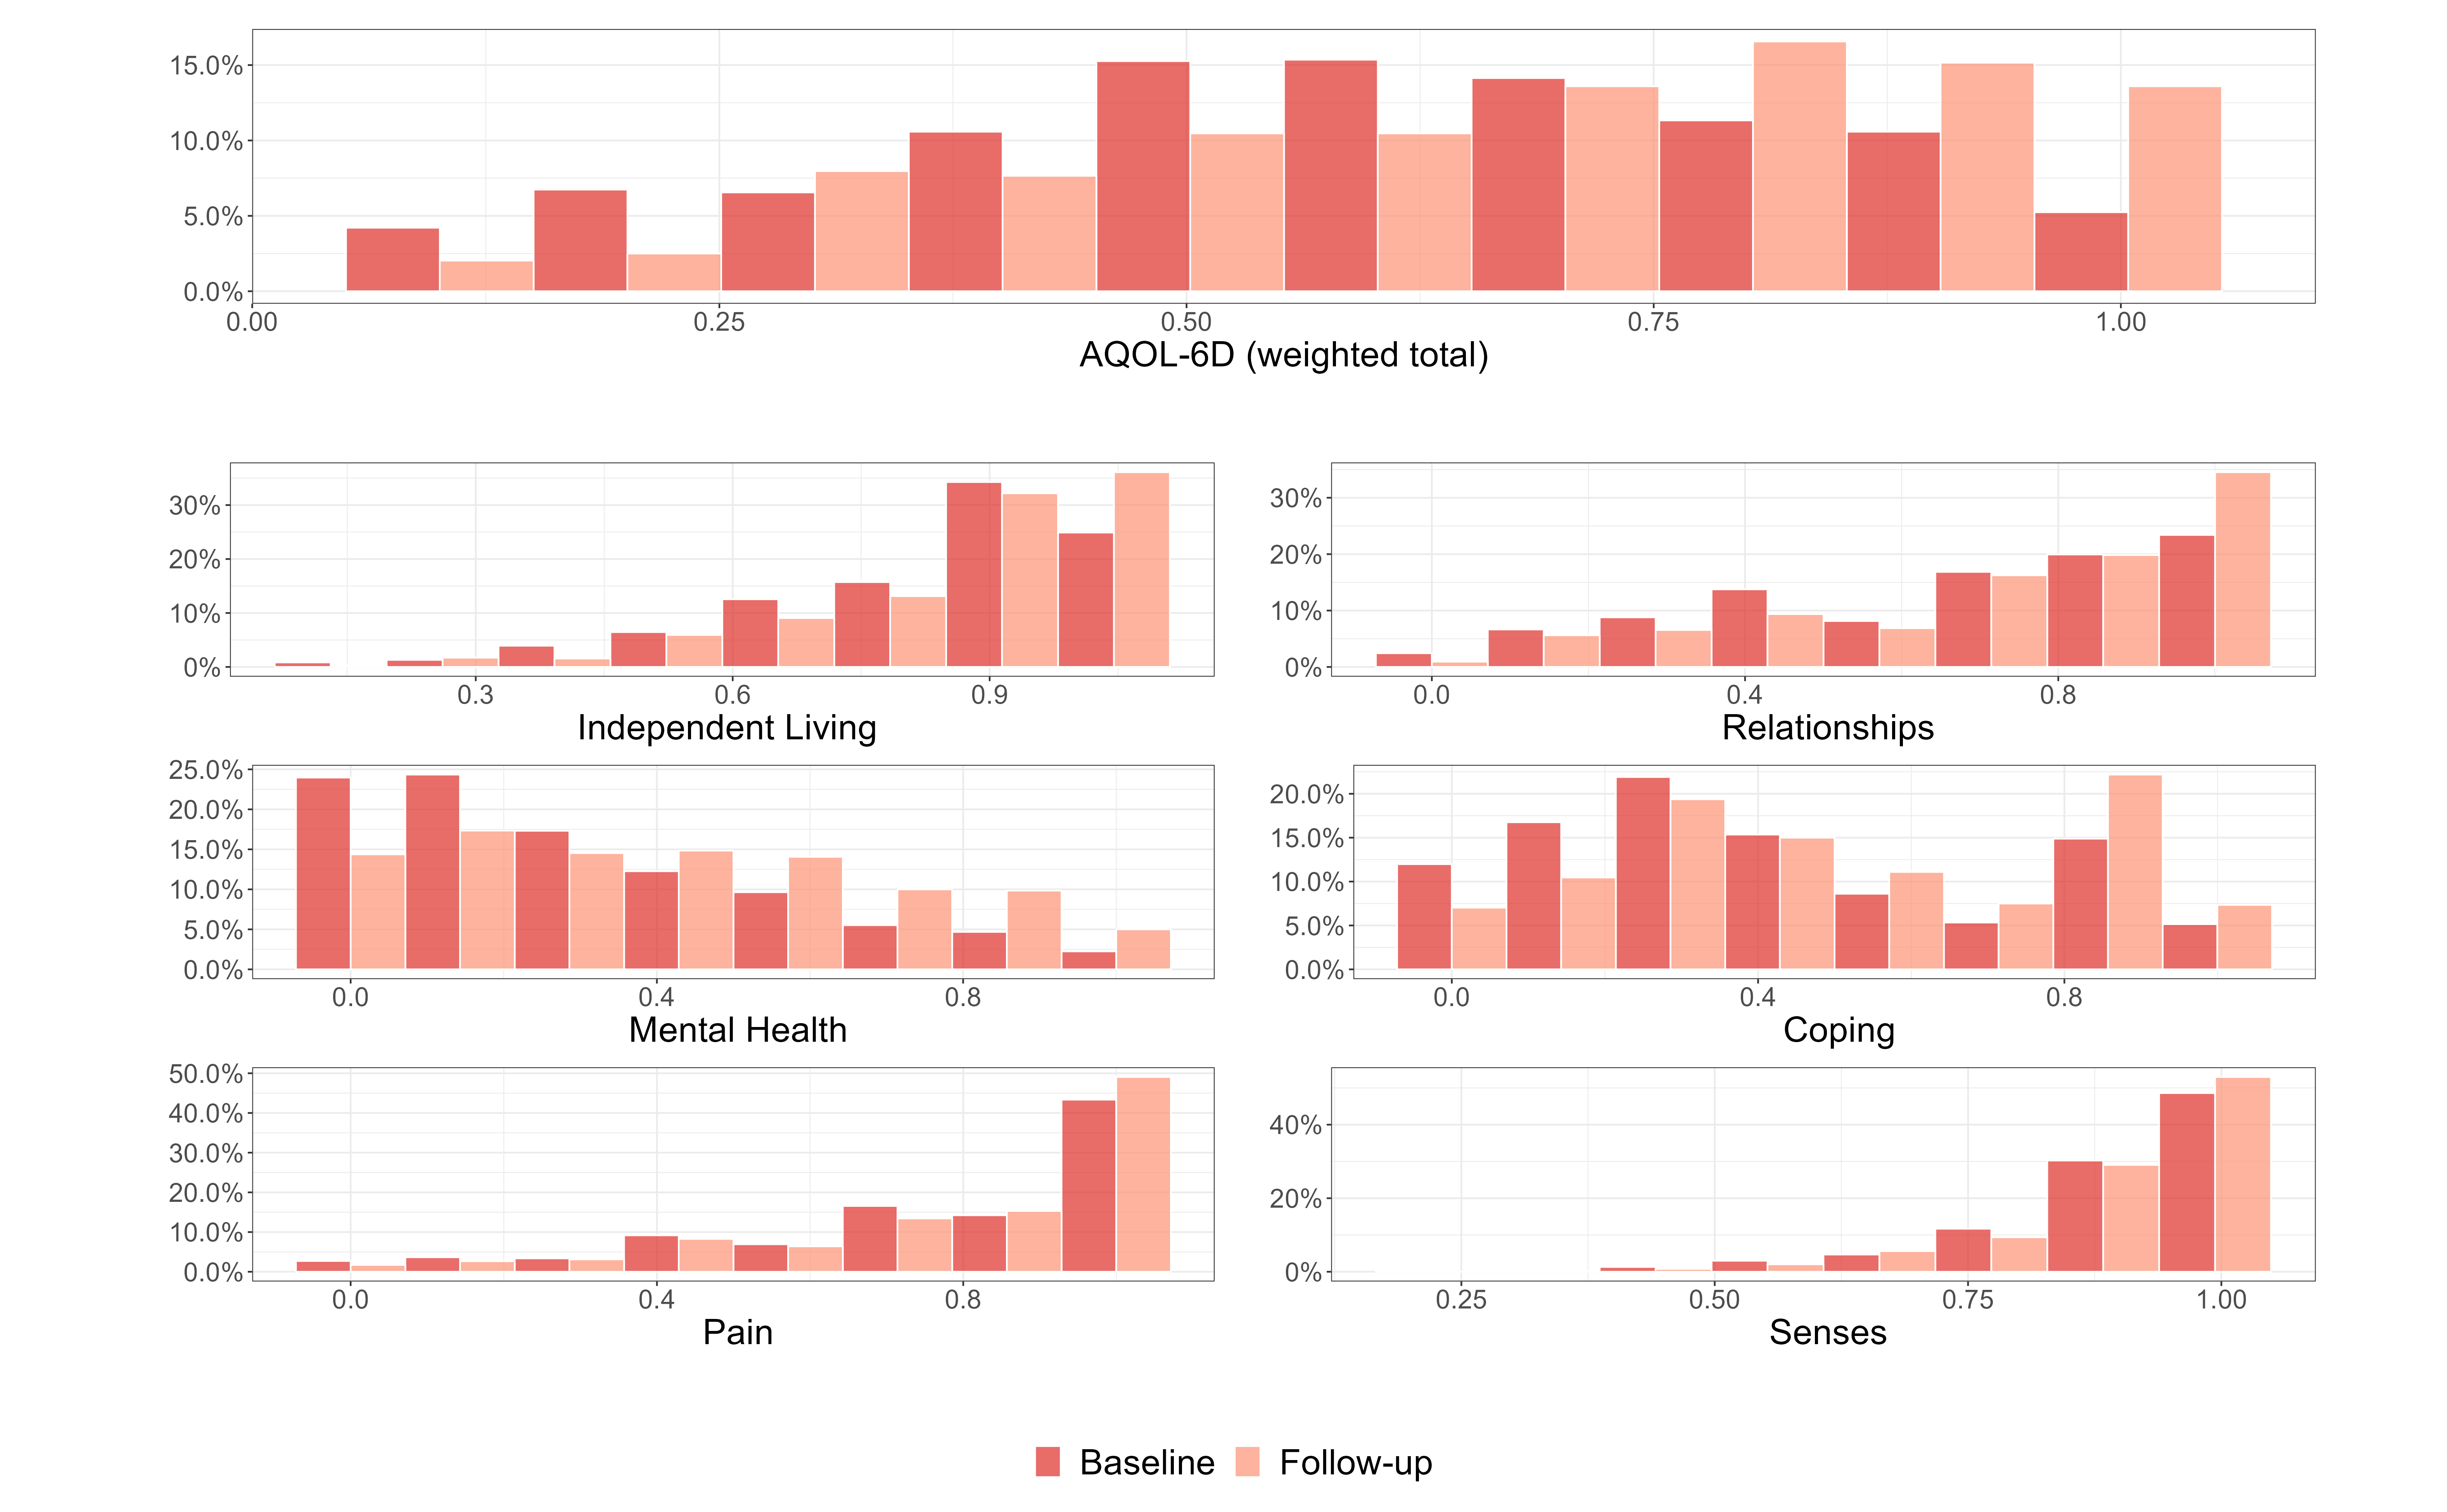
\includegraphics[width=400px]{combined_utl} \caption{Distribution of AQoL-6D domains}\label{fig:fig1}
\end{figure*}

\begin{figure*}
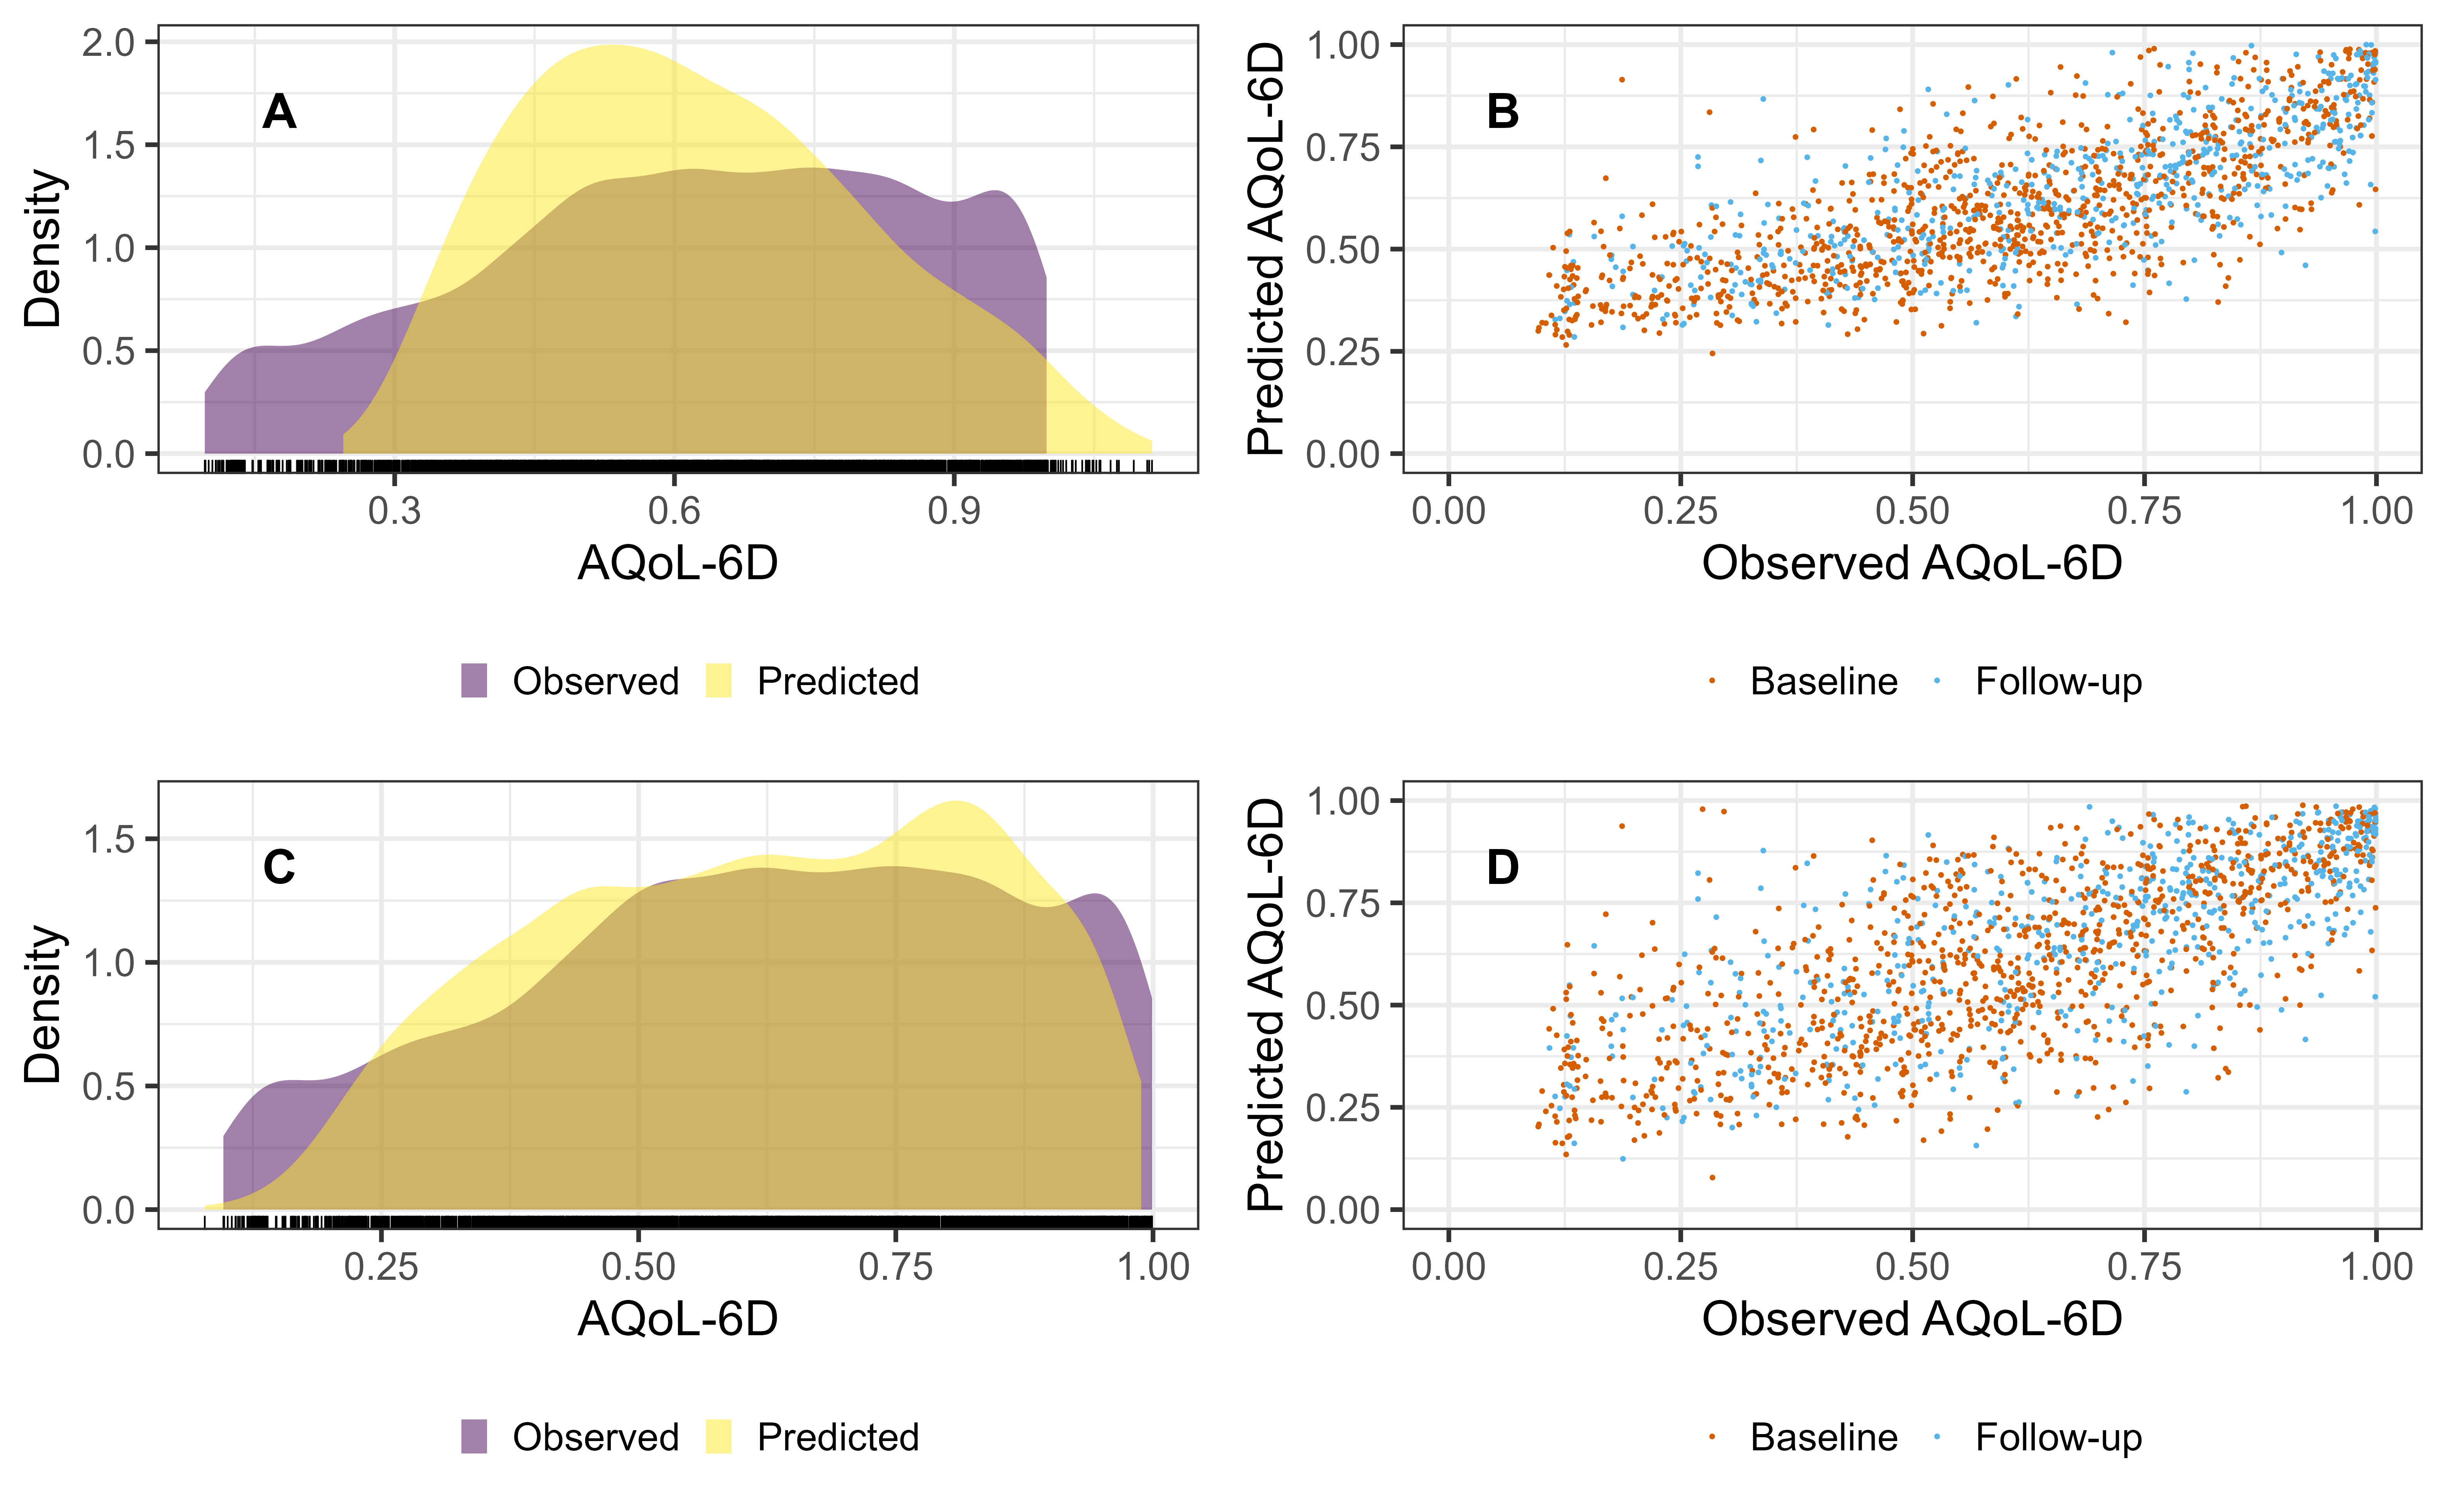
\includegraphics[width=400px]{dens_and_sctr} \caption{Comparison of observed and predicted AQoL-6D score from longitudinal model using PHQ-9 (A) Density plots of observed and predicted utility scores (GLMM (Gaussian distribution and log link)) (B) Scatter plots of observed and predicted utility scores by timepoint (GLMM (Gaussian distribution and log link)) (C) Density plots of observed and predicted results (LMM (complementary log log transformation)) (D) Scatter plots of observed and predicted results by timepoint (LMM (complementary log log transformation))}\label{fig:fig2}
\end{figure*}

\newpage

%\begin{acknowledgement}
%Insert the Acknowledgment text here.
%\end{acknowledgement}

\end{document}
